\documentclass[12pt,twoside]{book}

\usepackage[utf8]{inputenc}
\usepackage[turkish]{babel}
\usepackage[T1]{fontenc}

\usepackage{amsmath}
\usepackage{amssymb}
\usepackage{amsthm}
\usepackage{enumerate}
\usepackage[most]{tcolorbox}

\usepackage{circuitikz}
\usepackage{cancel}
\usepackage{bodegraph}
\usepackage{gensymb}

\usepackage{verbatim}
\usepackage{listings}
\usepackage{matlab-prettifier}

\usepackage{pgfplots}
\pgfplotsset{compat=newest}
\usepackage{pgffor}
\usepackage{xcolor}

\usepackage{tikz}
\usetikzlibrary{patterns}
\usetikzlibrary{babel}

\usetikzlibrary{shapes.misc}
\tikzset{cross/.style={cross out, draw=black, minimum size=2*(#1-\pgflinewidth), inner sep=0pt, outer sep=0pt},
%default radius will be 3pt. 
cross/.default={3pt}}
\usetikzlibrary{arrows}
\tikzset{
  arrow/.pic={\path[tips,every arrow/.try,->,>=#1] (0,0) -- +(.1pt,0);},
  pics/arrow/.default={triangle 90}
}

\usepackage{siunitx}
\usepackage{textcomp}

\usepackage{hyperref}
\hypersetup{
    colorlinks=true,
    linkcolor=blue,
    filecolor=magenta,      
    urlcolor=cyan,
    pdftitle={Kitap},
    pdfpagemode=FullScreen,
    }

\urlstyle{same}

\usepackage{graphicx}
\graphicspath{{svg-inkscape/}}
\usepackage{geometry}
\usepackage{subcaption}
\usepackage{tabularray}
\usepackage{tabularx}
\DefTblrTemplate{contfoot-text}{default}{Bir sonraki sayfada devam ediyor.} % Uzun Tablolar için alt kısım
\DefTblrTemplate{conthead-text}{default}{(Devam)} % Uzun Tablolar için üst kısım

\usepackage{lscape}

\usepackage{pgfplotstable}
\usepackage{booktabs}

\renewcommand{\chaptername}{Bölüm}
\renewcommand{\contentsname}{İçindekiler}
\renewcommand{\figurename}{Şekil}
\renewcommand{\tablename}{Tablo}
\renewcommand{\bibname}{Kaynaklar}
\renewcommand{\listfigurename}{Şekiller}
\renewcommand{\listtablename}{Tablolar}
\renewcommand{\appendixname}{Ek}
\renewcommand{\indexname}{Dizin}
\renewcommand{\partname}{Bölüm}
\renewcommand{\proofname}{İspat}

\begin{document}
\shorthandoff{=} % babel paketi hatasını gidermek için gerekli

\tableofcontents

\documentclass[12pt,hyperref=unicode]{beamer}

\usepackage[utf8]{inputenc}
\usepackage[turkish]{babel}
\usepackage[T1]{fontenc}

\usepackage{amsmath}
\usepackage{amssymb}
\usepackage{amsthm}
\usepackage{enumerate}
\usepackage{tikz}
\usepackage{transparent}
\usepackage{xcolor}
\usepackage{listings}
\usepackage{verbatim}
\usepackage{graphicx}

\usepackage{pgfplots}

\usetheme{Warsaw}
\usecolortheme{default}
\definecolor{nigdeyesili_acik}{RGB}{3, 150, 166}
\definecolor{nigdeyesili_koyu}{RGB}{143, 209, 217}
\setbeamercolor{structure}{fg=nigdeyesili_acik}

\author[Dr. Mehmet CANEVİ]{Arş.~Gör.~Dr.~M.~Canevi\inst{1}}

\institute{
    \inst{1}%
    Bilgisayar Mühendisliği\\
    Mühendislik Fakültesi
}
    
\date[2025] {Ders Notları, Ocak 2025}
\setbeamertemplate{footline}[frame number]

\logo{\transparent{0.4}
\includegraphics[width = 20mm]{logo}}

\definecolor{mGreen}{rgb}{0,0.6,0}
\definecolor{mGray}{rgb}{0.5,0.5,0.5}
\definecolor{mPurple}{rgb}{0.58,0,0.82}
\definecolor{backgroundColour}{rgb}{0.95,0.95,0.92}

\lstloadlanguages{C}
\lstdefinestyle{CStyle}{
    backgroundcolor=\color{backgroundColour},   
    commentstyle=\color{mGreen},
    keywordstyle=\color{red},
    numberstyle=\tiny\color{mGray},
    stringstyle=\color{mGreen},
    basicstyle=\footnotesize,
    breakatwhitespace=false,         
    breaklines=true,                 
    captionpos=b,                    
    keepspaces=true,                 
    numbers=left,                    
    numbersep=2pt,                  
    showspaces=false,                
    showstringspaces=false,
    showtabs=false,                  
    tabsize=1,
    language=C
}
\lstset{style=CStyle}

\AtBeginDocument{\shorthandoff{=}}
\title[Ders 1] {Kod Yazma, Kod Derleme. Değişken Tanımlama, Veri Tipleri. Operatörler.}
\begin{document}
%%%%%%%%%%%%%%%%%%%%%%%%%%%%%%%%%%%%%%%%%%%%%%%%%%%%%%%%%%%%%%%%%%%%%%%%%%%%%%%%
\frame{\titlepage}
\begin{frame}[fragile]{İçidekiler}
    \tableofcontents
\end{frame}
%%%%%%%%%%%%%%%%%%%%%%%%%%%%%%%%%%%%%%%%%%%%%%%%%%%%%%%%%%%%%%%%%%%%%%%%%%%%%%%%
\section{Kod yazma}
\begin{frame}[fragile]{Kod nedir?}
    \begin{itemize}
        \item Bilgisayar tanımı kapsamına giren cihazlara meramımızı anlatmak için yazılan yazıya \textbf{kod} diyebiliriz
        \item Bahsi geçen yazının bir dili olur ve buna kodun dili denir
        \item Bu ders kapsamında \verb|C| dilini kullanacağız
        \item \verb|C| dili insanın anlama şekline daha yakındır
        \item Makinenin anlama şekline yakın diline \textbf{makine dili} denir
    \end{itemize}
\end{frame}
%%%%%%%%%%%%%%%%%%%%%%%%%%%%%%%%%%%%%%%%%%%%%%%%%%%%%%%%%%%%%%%%%%%%%%%%%%%%%%%%
\begin{frame}[fragile]{Derleme nedir?}
    \begin{itemize}
        \item \verb|C| dilinden \textbf{makine dili}ne çeviri işlemidir
        \item Kod yazarken yapılan her güncelleme sonrası derlemeye ihtiyaç duyulur
        \item Derleme bazen hata ile sonuçlanabilir, muhtemel bir \textbf{imla hatası} sebep olabilir
        \item Derleme başarılı olmasına rağmen makine istenen davranışı göstermeyebilir(\textbf{mantıksal hata})
        \item \verb|Windows| için derleme(ve linkleme sonucu) \verb|exe| uzantılı bir dosya üretilir
    \end{itemize}
\end{frame}
%%%%%%%%%%%%%%%%%%%%%%%%%%%%%%%%%%%%%%%%%%%%%%%%%%%%%%%%%%%%%%%%%%%%%%%%%%%%%%%%
\begin{frame}[fragile]{Örnek bir kod}
    Örnek bir kod
    \lstinputlisting{lec1/main.c}
    şeklindedir.
\end{frame}
%%%%%%%%%%%%%%%%%%%%%%%%%%%%%%%%%%%%%%%%%%%%%%%%%%%%%%%%%%%%%%%%%%%%%%%%%%%%%%%%
\begin{frame}[fragile]{Örnek bir makine kodu}
    Örnek bir makine kodu
    \lstinputlisting{lec1/main.o}
    şeklindedir.
\end{frame}
%%%%%%%%%%%%%%%%%%%%%%%%%%%%%%%%%%%%%%%%%%%%%%%%%%%%%%%%%%%%%%%%%%%%%%%%%%%%%%%%
\begin{frame}[fragile]{Makine kodunun temeli}
    $4+6$ işlemini inceleyelim:
    \begin{equation}
        (0100)_2+(0110)_2=(1010)_2=10
    \end{equation}
    1 bitlik en basit toplama işlemi 
    \begin{figure}[!htb]
        \centering
        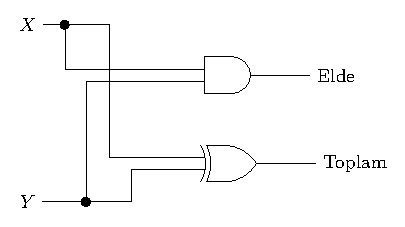
\includegraphics[width=0.5\textwidth]{lec1/xor}
    \end{figure}
    ile gösterilebilir. 4 bit için bu yapı temel alınıp gerçeklenebilir.
\end{frame}
%%%%%%%%%%%%%%%%%%%%%%%%%%%%%%%%%%%%%%%%%%%%%%%%%%%%%%%%%%%%%%%%%%%%%%%%%%%%%%%%
\begin{frame}[fragile]{Makine kodunun temeli(devam)}
    4 bit için bu yapı 
    \begin{figure}[!htb]
        \centering
        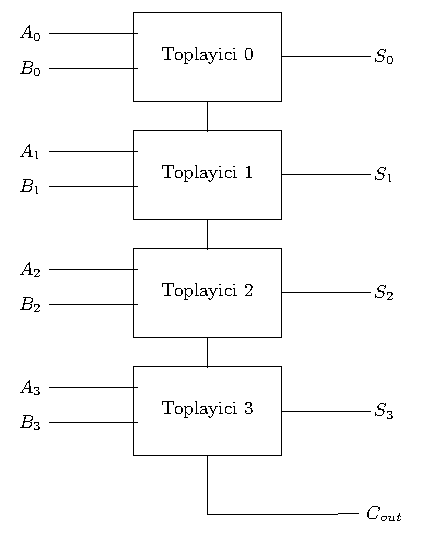
\includegraphics[height=0.6\textheight]{lec1/fulladder}
    \end{figure}
    şeklinde gösterilebilir.
\end{frame}
%%%%%%%%%%%%%%%%%%%%%%%%%%%%%%%%%%%%%%%%%%%%%%%%%%%%%%%%%%%%%%%%%%%%%%%%%%%%%%%%
\begin{frame}[fragile]{Makine kodunun temeli(devam)}
    \begin{itemize}
    \item 4 bitlik toplama devresi \textbf{çıkarma işlemi}, \textbf{çarpma işlemi} vb. işlemler ile aritmetik işlemci oluşturulabilmektedir. 
    \item Mantıksal işlemler için de tasarlanırsa ortaya Aritmetik Lojik Birim(ALB) ortaya çıkmaktadır. 
    \item Merkezi İşlemci Birimi(MİB) denilen karmaşık yapının başlangıcı denebilir.
    \end{itemize}
\end{frame}
%%%%%%%%%%%%%%%%%%%%%%%%%%%%%%%%%%%%%%%%%%%%%%%%%%%%%%%%%%%%%%%%%%%%%%%%%%%%%%%%
\section{Değişken tanımlama ve veri tipleri}
\begin{frame}[fragile]{Değişken isimleri}
    Değişkenler şu şekilde tanımlanmaktadır:
    \begin{lstlisting}
        veri_tipi degisken_adi;
        veri_tipi degisken_adi=ilk_deger;\end{lstlisting}
    Buradaki \lstinline{veri_tipi};
    \begin{itemize}
        \item \lstinline{int} 
        \item \lstinline{float}
        \item \lstinline{double}
        \item \lstinline{char}
    \end{itemize}
     olabilmektedir. \lstinline{degisken_adi} ise 
    \begin{itemize}
     \item türkçe karakter içermemelidir
     \item sadece harf veya alttire ile başlamalıdır
     \item özel karakterler(!,?,vb.) ve boşluk içermemelidir
     \item \lstinline{veri_tipi} anahtar kelimeleri olmamalıdır
    \end{itemize}
    kurallarına uymalıdır.
\end{frame}
%%%%%%%%%%%%%%%%%%%%%%%%%%%%%%%%%%%%%%%%%%%%%%%%%%%%%%%%%%%%%%%%%%%%%%%%%%%%%%%%
\begin{frame}[fragile]{Değişken tiplerinin anlamı}
    Değişkenler
    \begin{itemize}
     \item \lstinline{int} ingilizce \verb|integer| yani tam sayıdan gelmektedir \lstinline{-10,4} gibi
     \item \lstinline{float} ingilizcede kayan noktalı sayı(6-7 basamak) anlamındadır \lstinline{3.14f} gibi
     \item \lstinline{double} ingilizcede iki kat hassasiyet(15 basamak) anlamındadır \lstinline{3.14} gibi
     \item \lstinline{char} ingilizce \verb|character|'den gelir \lstinline{'c','x'} gibi
    \end{itemize}
    veri tipleri ile tanımlanabilmektedir ve 
    \begin{itemize}
        \item \lstinline{int var1=-10;} 
        \item \lstinline{float var2=3.14f;} 
        \item \lstinline{double var3=3.14;} 
        \item \lstinline{char var4='x';} 
    \end{itemize}
    olarak örneklendirilebilir.
\end{frame}
%%%%%%%%%%%%%%%%%%%%%%%%%%%%%%%%%%%%%%%%%%%%%%%%%%%%%%%%%%%%%%%%%%%%%%%%%%%%%%%%
\begin{frame}[fragile]{Çoklu değişken tanımlama}
    Birden fazla değişken
    \begin{itemize}
        \item \lstinline{int a,b,c=-10;} 
        \item \lstinline{float a=2.2,b,c=3.14f;} 
        \item \lstinline{double a,b,c=3.14;} 
        \item \lstinline{char a,b,c;a=b=c='x';}
    \end{itemize}
    şeklinde tanımlanabilir.
\end{frame}
%%%%%%%%%%%%%%%%%%%%%%%%%%%%%%%%%%%%%%%%%%%%%%%%%%%%%%%%%%%%%%%%%%%%%%%%%%%%%%%%
\begin{frame}[fragile]{Değişkenlerin yazdırılması}
    Değişkenler
    \begin{itemize}
        \item \lstinline{int var1=-10;printf("%d",var1);} 
        \item \lstinline{float var2=3.14f;printf("%f",var2);} 
        \item \lstinline{double var3=3.14;printf("%lf",var3);} 
        \item \lstinline{char var4='x';printf("%c",var4);}
        \item \lstinline{printf("%s","Bu bir cumledir.");}
    \end{itemize}
    ile ekrana yazdırılır.
\end{frame}
%%%%%%%%%%%%%%%%%%%%%%%%%%%%%%%%%%%%%%%%%%%%%%%%%%%%%%%%%%%%%%%%%%%%%%%%%%%%%%%%
\begin{frame}[fragile]{Sabit değerli değişkenler}
    Değeri değişmemesi gereken değişkenler
    \begin{itemize}
        \item \lstinline{const int SAAT_DK=60;} 
        \item \lstinline{const float PI_SAYISI=3.14;} 
    \end{itemize}
    şeklinde tanımlanır ve büyük harflerin kullanımı bir gelenektir. Dolayısıyla,
    \begin{itemize}
        \item \lstinline{SAAT_DK=120;} 
        \item \lstinline{PI_SAYISI=5.5;} 
    \end{itemize}
    hata verir.
\end{frame}
%%%%%%%%%%%%%%%%%%%%%%%%%%%%%%%%%%%%%%%%%%%%%%%%%%%%%%%%%%%%%%%%%%%%%%%%%%%%%%%%
\section{Operatörler}
\begin{frame}[fragile]{Matematiksel operatörler}
    Toplama ve çıkarma işlemi
    \begin{itemize}
        \item \lstinline{int a=4+5;int c=a-2;int d=a+c;} 
    \end{itemize}
    ile örneklendirilebilir. Matematiksel operatörler
    \begin{itemize}
        \item \lstinline{+,-} toplama, çıkarma 
        \item \lstinline{*,/} çarpma, bölme
        \item \lstinline{++,--} arttırma, azaltma 
        \item \lstinline{%} \verb|mod| operatörü (bölümden kalan)
        \item \lstinline{=} atama operatörü
    \end{itemize}
    şeklindedir.
\end{frame}
%%%%%%%%%%%%%%%%%%%%%%%%%%%%%%%%%%%%%%%%%%%%%%%%%%%%%%%%%%%%%%%%%%%%%%%%%%%%%%%%
\begin{frame}[fragile]{Matematiksel operatörler(devam)}
    Aşağıdaki operatörler tanımlıdır.
    \begin{itemize}
        \item \lstinline{x+=3;} \lstinline{x=x+3;} 
        \item \lstinline{x-=3;} \lstinline{x=x-3;} 
        \item \lstinline{x*=3;} \lstinline{x=x*3;} 
        \item \lstinline{x/=3;} \lstinline{x=x/3;} 
        \item \lstinline{x%=3;} \lstinline{x=x%3;} 
    \end{itemize}
\end{frame}
%%%%%%%%%%%%%%%%%%%%%%%%%%%%%%%%%%%%%%%%%%%%%%%%%%%%%%%%%%%%%%%%%%%%%%%%%%%%%%%%
\begin{frame}[fragile]{Karşılaştırma operatörleri}
    Aşağıdaki operatörler ile karşılaştırma başarılı ise 1 değilse sıfır değerini alır.
    \begin{itemize}
        \item \lstinline{x>y} Büyüktür
        \item \lstinline{x>=y} Büyük eşittir
        \item \lstinline{x<y} Küçüktür
        \item \lstinline{x<=y} Küçük eşittir
        \item \lstinline{x==y} Eşittir
        \item \lstinline{x!=y} Eşit değildir
    \end{itemize}
\end{frame}
%%%%%%%%%%%%%%%%%%%%%%%%%%%%%%%%%%%%%%%%%%%%%%%%%%%%%%%%%%%%%%%%%%%%%%%%%%%%%%%%
\begin{frame}[fragile]{Mantıksal operatörleri}
    Mantıksal operatörler
    \begin{itemize}
        \item \lstinline{sart1 && sart2} VE
        \item \lstinline{sart1 || sart2} VEYA 
        \item \lstinline{!sart} DEĞİLDİR 
    \end{itemize}
    olarak verilmiştir.
\end{frame}
%%%%%%%%%%%%%%%%%%%%%%%%%%%%%%%%%%%%%%%%%%%%%%%%%%%%%%%%%%%%%%%%%%%%%%%%%%%%%%%%
\end{document}
\chapter{Ayrıklaştırma}
Türevin geometrik yorumu 
\begin{equation}
    \frac{dy(t)}{dt}\approx\frac{\Delta y}{\Delta t}
\end{equation}
olmak üzere
\begin{equation}
\begin{split}
    \frac{dy(t)}{dt}&\approx\frac{\Delta y}{\Delta t}\\
    &\approx\frac{y((k+1)T)-y(kT)}{(k+1)T-kT}\\
    &\approx\frac{y((k+1)T)-y(kT)}{T}
\end{split}
\end{equation}
elde edilir. Ayrık bir sinyalin türevi ardışık değerler farkının örnekleme zamanına oranı ile hesaplanabilmektedir. Örneğin, $y(kT)=\sin(kT)$ ve $T=0.1$ olmak üzere
\begin{equation}
    \frac{y((k+1)T)-y(kT)}{T}=10(\sin((k+1)0.1)-\sin(0.1k))
\end{equation}
ve dolayısıyla
\begin{equation}
\begin{split}
    \{10\sin(0.1),10(\sin(0.2)-\sin(0.1)),10(\sin(0.3)-\sin(0.2)),\cdots\}\\
    \{0.9983,0.9884, 0.9685,\cdots\}
\end{split}
\end{equation}
elde edilir. $y(kT)=\sin(kT)$ sinyalinin türevinin $\frac{d\sin(t)}{dt}=\cos(t)$ olduğu bilindiğinden
\begin{equation}
    \begin{split}
        \{cos(0.1),cos(0.2),cos(0.3),\cdots\}\\
        \{ 0.9950,0.9801,0.9553,\cdots\}
    \end{split}
\end{equation}
elde edilir ve ayrık türev ile benzer değerler olduğu görülmektedir. Bu yaklaşıklığın türeve yakınsaması için örnekleme zamanı $T$ daha küçük seçilmelidir. 
\begin{equation}
    \frac{dq(t)}{dt}=x
\end{equation}
olmak üzere
\begin{equation}
\begin{split}
    \frac{dq(t)}{dt}&=x\\
    dq(t)&=xdt\\
    \int dq(t)&=\int xdt\\
    q(t)&=\int xdt
\end{split}
\end{equation}
elde edilir. Buradan hareketle,
\begin{equation}
    \begin{split}
        \frac{\Delta q}{\Delta t}&=x\\
        \frac{q((k+1)T)-q(kT)}{(k+1)T-kT}&=x\\
        \frac{q((k+1)T)-q(kT)}{T}&=x\\
        q((k+1)T)-q(kT)&=xT\\
        q((k+1)T)&=q(kT)+xT
    \end{split}
\end{equation}
ifadesi bulunur. Ayrık zamanda integral birikimli toplama karşılık gelmektedir. Bu karşılıklar Zero Order Hold(ZOH) ile elde edilmiştir. ZOH örnekleme zamanı boyunca değerlerin sabit olduğu varsayımına dayanmaktadır. Bu durum
\begin{equation}
    x(t)=x(kT),\quad kT\leq t\leq (k+1)T
\end{equation}
ile ifade edilebilir. ZOH için transfer fonksiyonu elde etmek amacıyla girişe $\delta(t)$ birim darbe fonksiyonu uygulanırsa çıkışında $u(t)-u(t-T)$ elde edilir. Bu durumda S tanım bölgesinde çıkış ifadesi
\begin{equation}
\begin{split}
    \mathcal{L}\{u(t)-u(t-T)\}&=\mathcal{L}\{u(t)\}-\mathcal{L}\{u(t-T)\}\\
    &=\mathcal{L}\{u(t)\}-e^{-sT}\mathcal{L}\{u(t)\}\\
    &=\frac{1}{s}-e^{-sT}\frac{1}{s}\\
    &=(1-e^{-sT})\frac{1}{s}
\end{split}
\end{equation}
şeklindedir. ZOH transfer fonksiyonu ile bir $G(s)$ sistemi birlikte Z dönüşümü yapılmalıdır. Örneğin,
\begin{equation}
    G(s)=\frac{1}{s+1}
    \label{eqn:ornek_sistem}
\end{equation}
sistemi ayrıklaştırılmak istensin. Bu durumda $G_{ZOH}(s)G(s)$ ayrıklaştırılmalıdır. Bu sebeple,
\begin{equation}
    L(s)=G_{ZOH}(s)G(s)=\frac{1-e^{-sT}}{s(s+1)}
\end{equation}
ifadesi Z tanım bölgesine
\begin{equation}
\begin{split}
    \mathcal{Z}\{L(s)\}&=\mathcal{Z}\left\{\frac{1-e^{-sT}}{s(s+1)}\right\}\\
    &=\mathcal{Z}\{1-e^{-sT}\} \mathcal{Z}\left\{\frac{1}{s(s+1)} \right\}\\
    &=(1-z^{-1}) \left(\mathcal{Z}\left\{\frac{1}{s}-\frac{1}{s+1} \right\}\right)\\
    &=\left(1-\frac{1}{z}\right) \left(\mathcal{Z}\left\{\frac{1}{s}\right\}-\mathcal{Z}\left\{\frac{1}{s+1} \right\}\right)\\
    &=\frac{z-1}{z} \left(\frac{z}{z-1}-\frac{z}{z-e^{-1}}\right)\\
    &=\left(1-\frac{z-1}{z-e^{-1}}\right)\\
    &=\frac{1-e^{-1}}{z-e^{-1}}
\end{split}\label{eqn:ornek_sistem_zoh}
\end{equation}
olarak dönüştürülür.

First Order Hold(FOH) yöntemi ise
\begin{equation}
    x(t)=x(kT)+\frac{t-kT}{T}(x((k+1)T)-x(kT)),\quad kT\leq t\leq (k+1)T
\end{equation}
olarak tanımlanır. Eşitliğin sağ tarafı $t=kT$ için $x(kT)$, $t=(k+0.5)T$ için 
\begin{equation}
\begin{split}
    x(t)&=x(kT)+\frac{t-kT}{T}(x((k+1)T)-x(kT)),\quad kT\leq t\leq (k+1)T\\
    &=x(kT)+\frac{kT+0.5T-kT}{T}(x((k+1)T)-x(kT))\\
    &=x(kT)+0.5(x((k+1)T)-x(kT))\\
    &=x(kT)+0.5x((k+1)T)-0.5x(kT)\\
    &=0.5x((k+1)T)+0.5x(kT)
\end{split}
\end{equation}
ve $t=(k+1)T$ için ise 
\begin{equation}
    \begin{split}
        x(t)&=x(kT)+\frac{t-kT}{T}(x((k+1)T)-x(kT)),\quad kT\leq t\leq (k+1)T\\
        x(t)&=x(kT)+\frac{(k+1)T-kT}{T}(x((k+1)T)-x(kT))\\
        x(t)&=x(kT)+x((k+1)T)-x(kT)\\
        x(t)&=x((k+1)T)
    \end{split}
\end{equation}
olarak elde edilir. Görüldüğü üzere ZOH yönteminin aksine $T$ süre boyunca değerler değişmektedir. FOH için birim darbe yanıtı
\begin{equation}
    x(t)=\begin{cases}
        t+\frac{1}{T} & 0\leq t\leq \frac{1}{T}\\
        -t+\frac{1}{T} & \frac{1}{T}\leq t\leq \frac{2}{T}\\
        0 & t>\frac{2}{T}
    \end{cases}
\end{equation}
ve işlem kolaylığı açısından $T=1$ alınırsa 
\begin{equation}
    x(t)=(1-t)u(2-t)+2tu(1-t)
\end{equation}
şeklindedir. S dönüşümü sonucu
\begin{equation}
\begin{split}
    \mathcal{L}\{x(t)\}&=\mathcal{L}\{(1-t)u(2-t)\}+\mathcal{L}\{2tu(1-t)\}\\
    &=\mathcal{L}\{(1-t)(1-u(t-2))\}+\mathcal{L}\{2t(1-u(t-1))\}\\
    &=\mathcal{L}\{(1-t)\}-\mathcal{L}\{(1-t)u(t-2)\}+\mathcal{L}\{2t\}-\mathcal{L}\{2tu(t-1)\}\\
    &=\mathcal{L}\{(1+t)\}+\mathcal{L}\{(t-1)u(t-2)\}-\mathcal{L}\{2tu(t-1)\}\\
    &=\mathcal{L}\{(1+t)\}+\mathcal{L}\{(t-1)u(t-2)\}-\mathcal{L}\{(2t-2+2)u(t-1)\}\\
    &=\mathcal{L}\{(1+t)\}+\mathcal{L}\{(t-1-1+1)u(t-2)\}-\mathcal{L}\{(2t-2+2)u(t-1)\}\\
    &=\mathcal{L}\{(1+t)\}+\mathcal{L}\{(t-2)u(t-2)+u(t-2)\}-\mathcal{L}\{(2t-2)u(t-1)+2u(t-1)\}\\
    &=\frac{1}{s}+\frac{1}{s^2}+\frac{e^{-2s}}{s^2}+\frac{e^{-2s}}{s}-2\frac{e^{-s}}{s^2}-\frac{2e^{-s}}{s}\\
    &=\frac{1-2e^{-s}+e^{-2s}}{s}+\frac{1-2e^{-s}+e^{-2s}}{s^2}\\
    &=\frac{(1-e^{-s})^2}{s}+\frac{(1-e^{-s})^2}{s^2}\\
    &=\frac{(1-e^{-s})^2}{s^2}(s+1)\\
\end{split}
\end{equation}
elde edilir. FOH için transfer fonksiyonu
\begin{equation}
    \begin{split}
        G_{FOH}(s)&=\frac{(1-e^{-s})^2}{T^2s^2}\frac{Ts+1}{T}\\
        &=G_{ZOH}^2(s)\frac{Ts+1}{T}
\end{split}
\end{equation}
şeklindedir. Örneğin daha önce Denklem~\ref{eqn:ornek_sistem} ile verilen sistemi FOH yöntemi ve yine aynı örnekleme zamanı ile ayrıklaştırmak gerekirse
\begin{equation}
\begin{split}
    L(s)&=\frac{1}{s+1}G_{FOH}(s)\\
    &=\frac{1}{s+1}\frac{(1-e^{-s})^2}{T^2s^2}\frac{Ts+1}{T}\\
    &=\frac{1}{s+1}\frac{(1-e^{-s})^2}{s^2}(s+1)\\
    &=\frac{(1-e^{-s})^2}{s^2}
\end{split}
\end{equation}
ifadesi Z dönüşümüne tabi tutulmalıdır. Dolayısıyla,
\begin{equation}
    \begin{split}
        G(z)&=\mathcal{Z}\left\{\frac{(1-e^{-s})^2}{s^2}\right\}\\
        &=\mathcal{Z}\{(1-e^{-s})^2\}\mathcal{Z}\left\{\frac{1}{s^2}\right\}\\
        &=\left(1-z^{-1}\right)^2\frac{Tz}{(z-1)^2}\\
        &=\left(\frac{z-1}{z}\right)^2\frac{z}{(z-1)^2}\\
        &=\frac{1}{z}
    \end{split}\label{eqn:ornek_sistem_foh}
\end{equation}
elde edilir. Görüldüğü üzere, birim gecikme elde edilmiştir.

\begin{enumerate}
    \item $x(t)=sin(t)$ fonksiyonunun türevini hesaplayıp çiziniz.
    \begin{lstlisting}[style=Matlab-editor]
    t=0:0.1:10;
    xt=sin(t);
    dxt=zeros(size(t));
    T=t(2)-t(1);
    for i=2:length(t)
        dxt(i)=(xt(i)-xt(i-1))/T;
    end
    figure(1);clf;hold on;grid on;xlabel("Zaman(s)");ylabel("x(t)");title("sin(t) ve turevi");
    plot(t,xt,'k','LineWidth',2);
    plot(t,dxt,'r','LineWidth',2);
    \end{lstlisting}
    Şekil~\ref{fig:lec2_plot1}'de $sin(t)$ ve türevi gösterilmiştir.
    \begin{figure}[!htb]
        \centering
        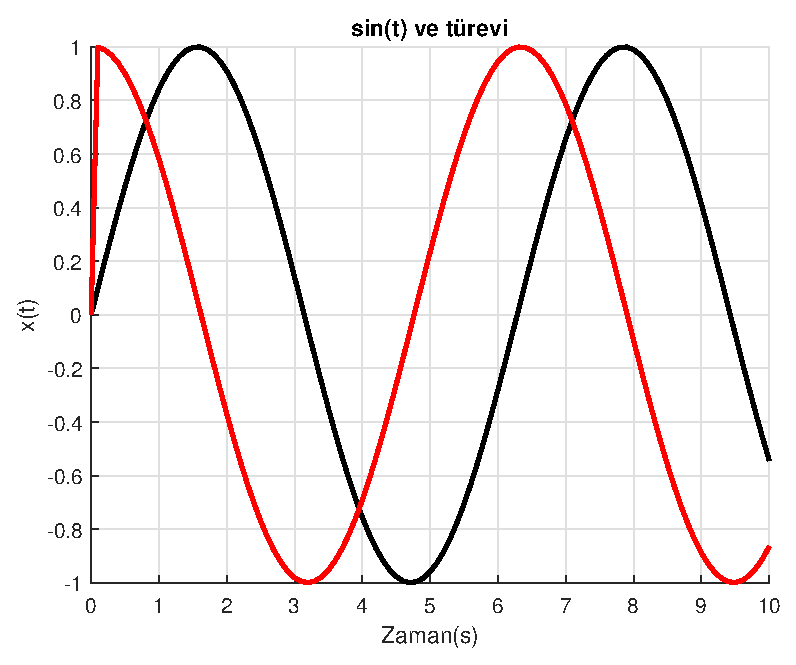
\includegraphics[width=0.5\textwidth]{img/lec2_plot1}
        \caption{$sin(t)$ ve türevinin karşılaştırılması($T=0.1$)}
        \label{fig:lec2_plot1}
    \end{figure}

    Şekil~\ref{fig:lec2_plot2}'de daha düşük bir örnekleme zamanı seçilmiştir ve bu sebeple gerek sinyal gerekse türevi düşük kalitededir.
    \begin{figure}[!htb]
        \centering
        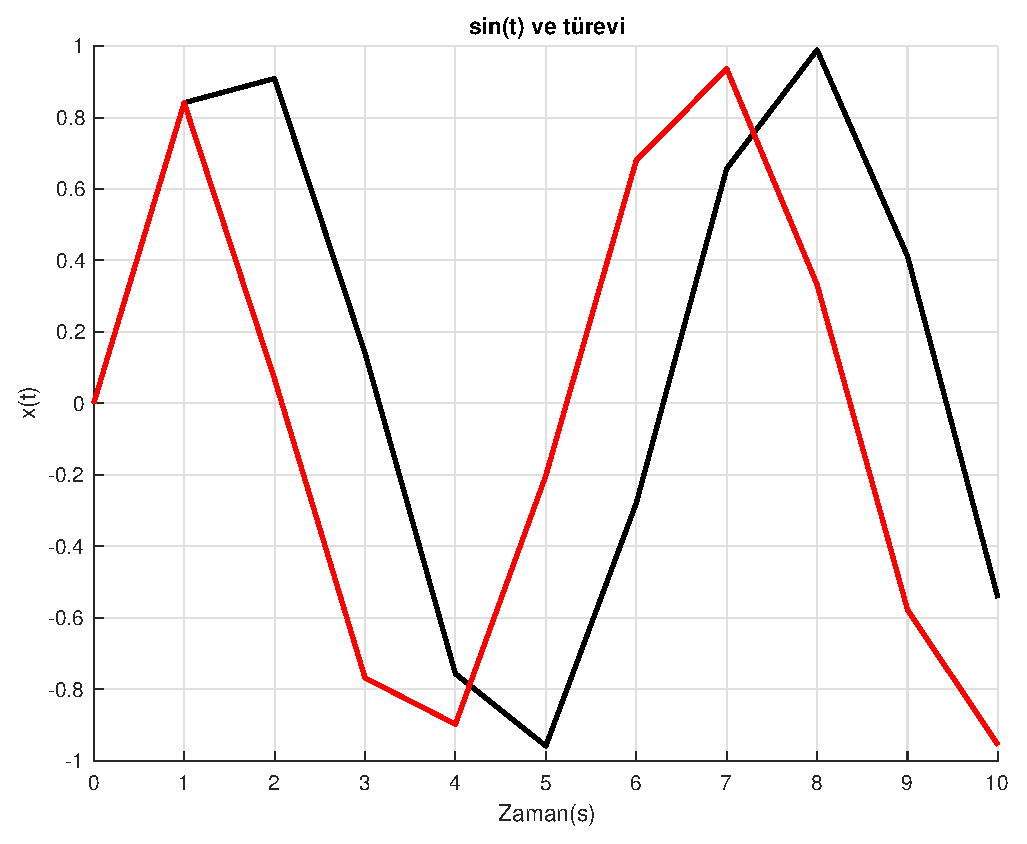
\includegraphics[width=0.5\textwidth]{img/lec2_plot2}
        \caption{$sin(t)$ ve türevinin karşılaştırılması($T=1$)}
        \label{fig:lec2_plot2}
    \end{figure}
    \item $x(t)=e^{-t}$ sinyalinin integralini hesaplayınız ve çizdiriniz.
    \begin{lstlisting}[style=Matlab-editor]
    t=0:1:10;
    xt=exp(-t);
    q=zeros(size(t));
    T=t(2)-t(1);
    for i=2:length(t)
        q(i)=q(i-1)+xt(i-1)*T;
    end
    figure(1);clf;hold on;grid on;xlabel("Zaman(s)");ylabel("x(t)");title("sin(t) ve integrali");
    plot(t,xt,'k','LineWidth',2);
    plot(t,q,'r','LineWidth',2);
    \end{lstlisting}
    Şekil~\ref{fig:lec2_plot3}'de integral çizdirilmiştir.
    \begin{figure}[!htb]
        \centering
        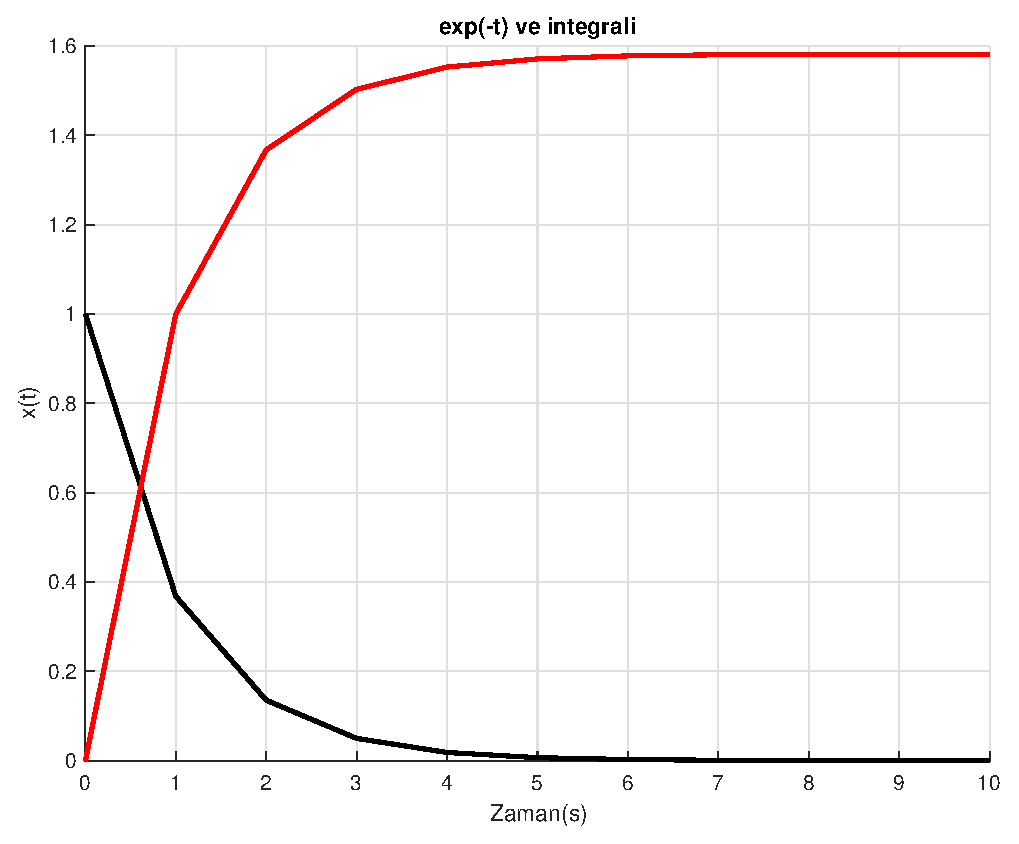
\includegraphics[width=0.5\textwidth]{img/lec2_plot3}
        \caption{$sin(t)$ ve integralinin karşılaştırılması($T=1$)}
        \label{fig:lec2_plot3}
    \end{figure}
    \item ZOH yöntemini kullanarak $T=1$ olmak üzere $x(kT)=1$ sinyalini veri tutucunu çıkışını çizdiriniz.
    \begin{lstlisting}[style=Matlab-editor]
    T=1;
    t=0:T:3;
    xt=[1,2,-1,3];
    
    tnew=0:0.01:4;
    yt=zeros(size(tnew));
    for i=1:length(t)
        for j=1:100
            yt(100*(i-1)+j)=xt(i);
        end
    end
    figure(1);clf;hold on;grid on;xlabel("Zaman(s)");ylabel("x(t)");title("ZOH ornegi");
    stem(t,xt,'k','LineWidth',2);
    plot(tnew,yt,'r','LineWidth',2);
    \end{lstlisting}
    Şekil~\ref{fig:lec2_plot4}'de ZOH işleminin sonucu gösterilmiştir.
    \begin{figure}[!htb]
        \centering
        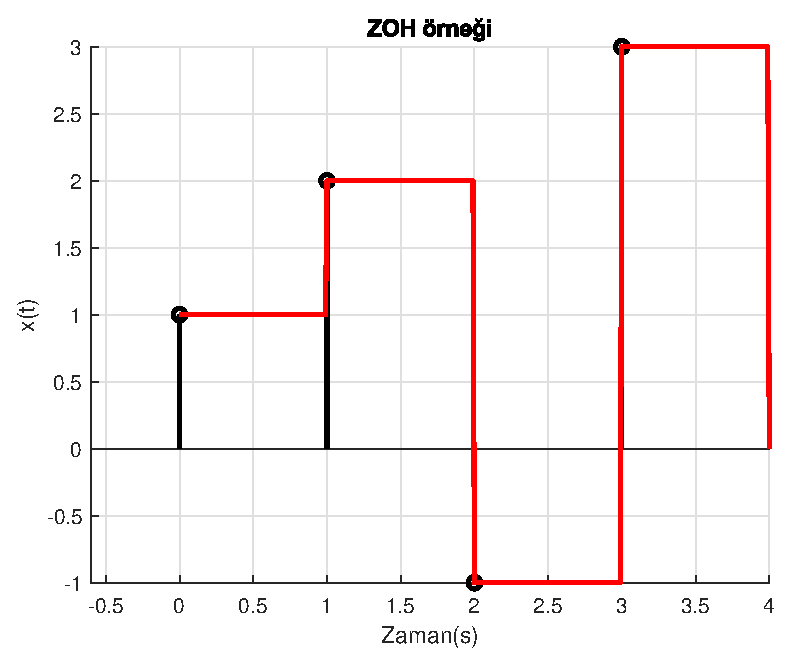
\includegraphics[width=0.5\textwidth]{img/lec2_plot4}
        \caption{ZOH örneği}
        \label{fig:lec2_plot4}
    \end{figure}
\end{enumerate}
\chapter{Fark Denklemleri}
Örnek sistemin ZOH yöntemi ile elde edilen ve Denklem~\ref{eqn:ornek_sistem_zoh} ile verilen sistem için
\begin{equation}
\begin{split}
    G_{ZOH}(z)&=\frac{1-e^{-1}}{z-e^{-1}}\\
    &=\frac{(1-e^{-1})z^{-1}}{1-e^{-1}z^{-1}}\\
    \frac{y(z)}{u(z)}&=\frac{(1-e^{-1})z^{-1}}{1-e^{-1}z^{-1}}\\
    y(z)(1-e^{-1}z^{-1})&=\frac{(1-e^{-1})z^{-1}u(z)}{1-e^{-1}z^{-1}}\\
    y(z)-y(z-1)e^{-1}&=(1-e^{-1})u(z-1)\\
    y(z)&=y(z-1)e^{-1}+(1-e^{-1})u(z-1)\\
    y(z)&=0.3679y(z-1)+0.6321u(z-1)
\end{split}
\end{equation}
elde edilir. Z tanım bölgesinde tanımlı transfer fonksiyonundan fark denklemine geçişe örnektir. Fark denklemleri programlama dilleri ile kolaylıkla gerçeklenebilmektedir.
\begin{lstlisting}
u=ones(1,length(t));
y=zeros(1,length(t));

for i=2:length(t)
    y(i)=exp(-T)*y(i-1)+(1-exp(-T))*u(i);
end\end{lstlisting}
Benzer şekilde FOH yöntemi ile elde edilen ve Denklem~\ref{eqn:ornek_sistem_foh} ile verilen ifade için
\begin{equation}
    \begin{split}
        G_{FOH}(z)&=\frac{1}{z}\\
        \frac{y(z)}{u(z)}&=z^{-1}\\
        y(z)&=u(z-1)
    \end{split}
\end{equation}
elde edilir.
Yay-Kütle-Damper sistemi için dinamikleri ifade eden denklem
\begin{equation}
    m\ddot{x}(t)+b\dot{x}(t)+kx(t)=u(t)
\end{equation}
olarak verilmiştir. Bu diferansiyel denklem S tanım bölgesine dönüştürülürse
\begin{equation}
\begin{split}
    ms^2X(s)+b sX(s)+kX(s)&=U(s)\\
    (ms^2+b s+k)X(s)&=U(s)\\
    \frac{X(s)}{U(s)}=\frac{1}{ms^2+b s+k}
\end{split}
\end{equation}
elde edilir.

\end{document}
